\documentclass{article}

%%% Choosing the margins of the document %%%
\usepackage{geometry}
\geometry{a4paper, portrait, margin=1in}
%%% Package to make sure figures are in right section %%%
\usepackage[section]{placeins}
%%% package for colours
\usepackage{color}
\usepackage{lscape}

\usepackage{Sweave}
\begin{document}
\Sconcordance{concordance:EstimatingRatesFromUNPD.tex:/home/mike/POPART_NEW/IBM_simul/data/RAW_PRIORS/SOURCED_FROM_LITERATURE/Analysing_UNPD_estimates_demographic_params/EstimatingRatesFromUNPD.Rnw:%
1 11 1 1 0 9 1 1 28 3 1 1 46 1 1 1 21 1 26 3 0 1 6 1 2 1 21 1 24 3 0 1 %
6 1 2 3 1 1 21 1 25 3 0 1 6 1 2 1 20 1 24 3 0 1 6 1 2 71 1 1 3 14 0 1 1 %
14 0 1 2 14 0 1 1 14 0 1 3 7 1 1 3 2 0 1 1 4 0 1 3 5 1 2 20 22 1 1 22 %
14 1}


%%% Some options to make the R code look nicer in Sweave %%%
\DefineVerbatimEnvironment{Sinput}{Verbatim} {xleftmargin=2em}
\DefineVerbatimEnvironment{Soutput}{Verbatim}{xleftmargin=2em}
\DefineVerbatimEnvironment{Scode}{Verbatim}{xleftmargin=2em}
\fvset{listparameters={\setlength{\topsep}{0pt}}}
\renewenvironment{Schunk}{\vspace{\topsep}}{\vspace{\topsep}}

%%%%%%%%%%%%%%%%%%%%%%%%%%%%%%%%%%%%%%%%%%%%%%%%

\section*{Mortality rates}




\begin{Schunk}
\begin{Soutput}
NULL
\end{Soutput}
\end{Schunk}


\begin{Schunk}
\begin{Soutput}
NULL
\end{Soutput}
\end{Schunk}


%%%%%%%%%%%%%%%%%%%%%%%%%%%%%%%%%%%%%%%


\begin{Schunk}
\begin{Soutput}
NULL
\end{Soutput}
\end{Schunk}


\begin{Schunk}
\begin{Soutput}
NULL
\end{Soutput}
\end{Schunk}


%%%%%%%%%%%%%%%%%%%%%%%%%%%%%%%%%%%%%%%%

\begin{figure}
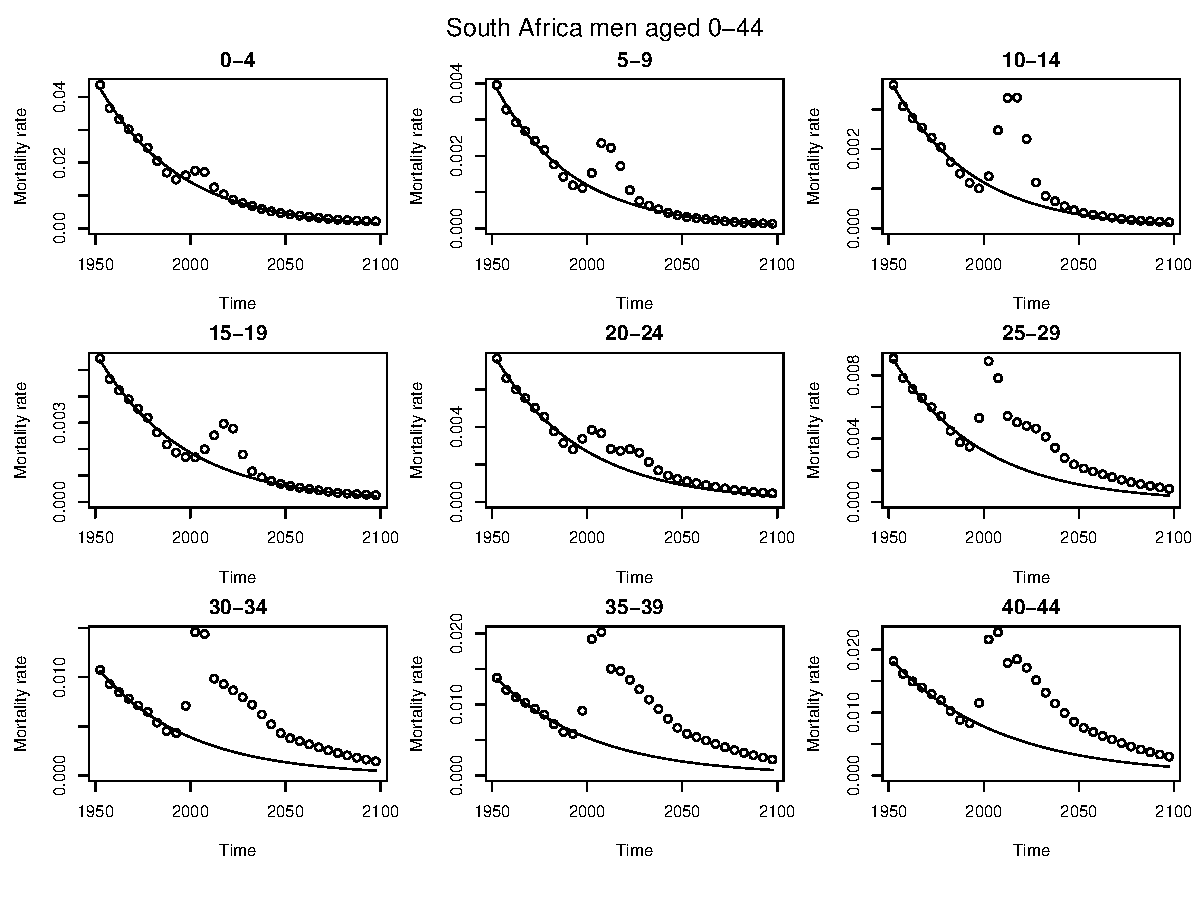
\includegraphics[width=16cm,height=16cm]{EstimatingRatesFromUNPD-MortalitySAMen1} 

\caption{Mortality rates for men in South Africa over time by 5 year age groups. Circles show UNPD estimates (including HIV mortality), lines show estimate based on a log-linear model for each age group.}
\label{MortalitySAmen1}
\end{figure}


\begin{figure}
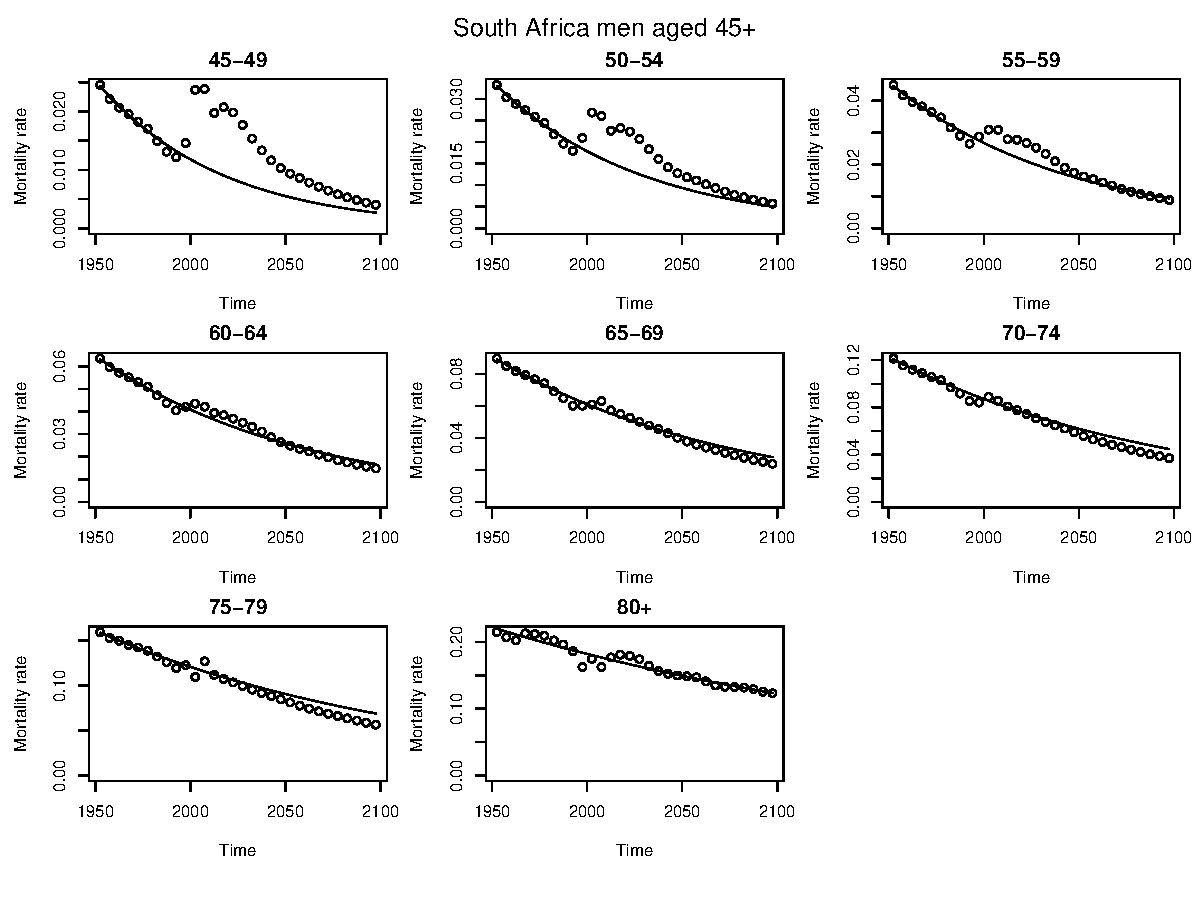
\includegraphics[width=16cm,height=16cm]{EstimatingRatesFromUNPD-MortalitySAMen2} 

\caption{Mortality rates for men in South Africa over time by 5 year age groups (cont). Circles show UNPD estimates (including HIV mortality), lines show estimate based on a log-linear model for each age group.}
\label{MortalitySAmen1}
\end{figure}


\begin{figure}
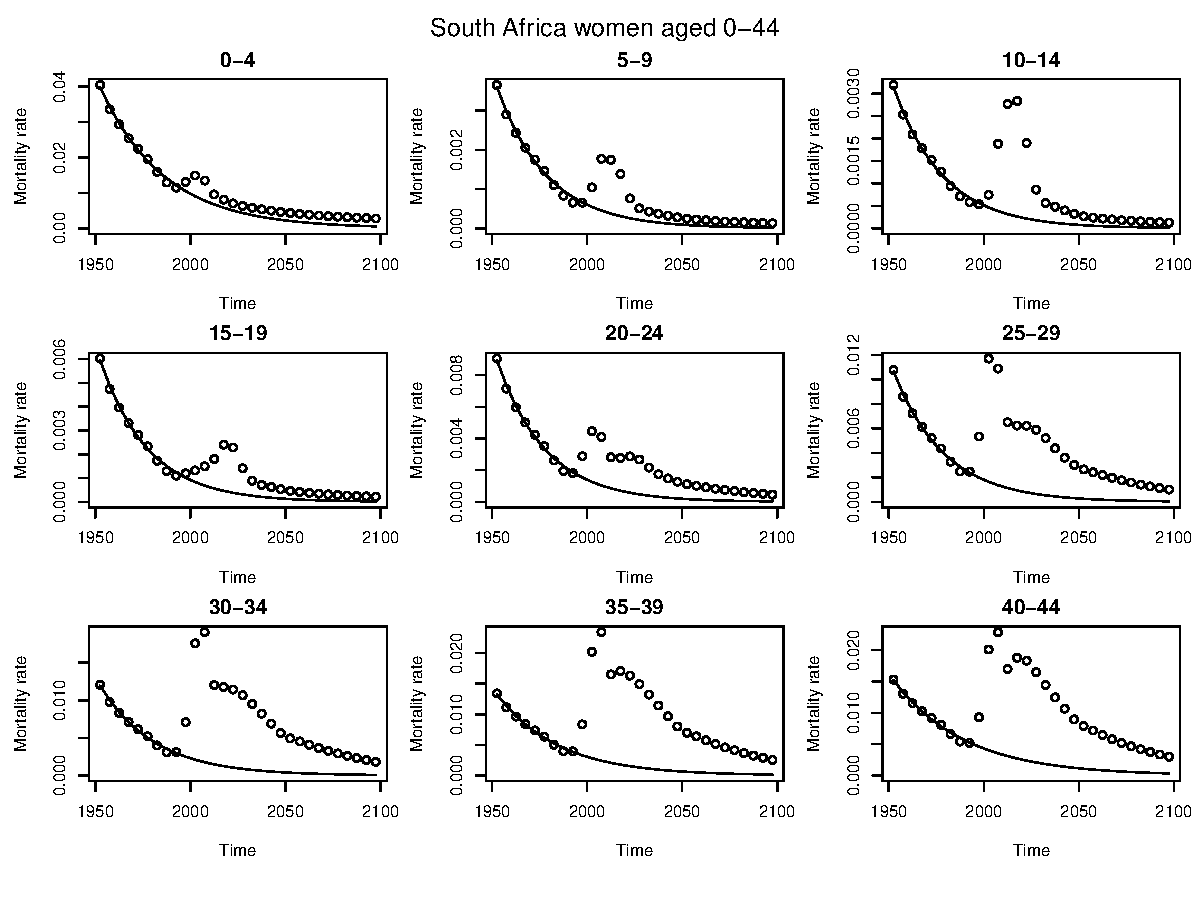
\includegraphics[width=16cm,height=16cm]{EstimatingRatesFromUNPD-MortalitySAWomen1} 

\caption{Mortality rates for women in South Africa over time by 5 year age groups. Circles show UNPD estimates (including HIV mortality), lines show estimate based on a log-linear model for each age group.}
\label{MortalitySAmen1}
\end{figure}


\begin{figure}
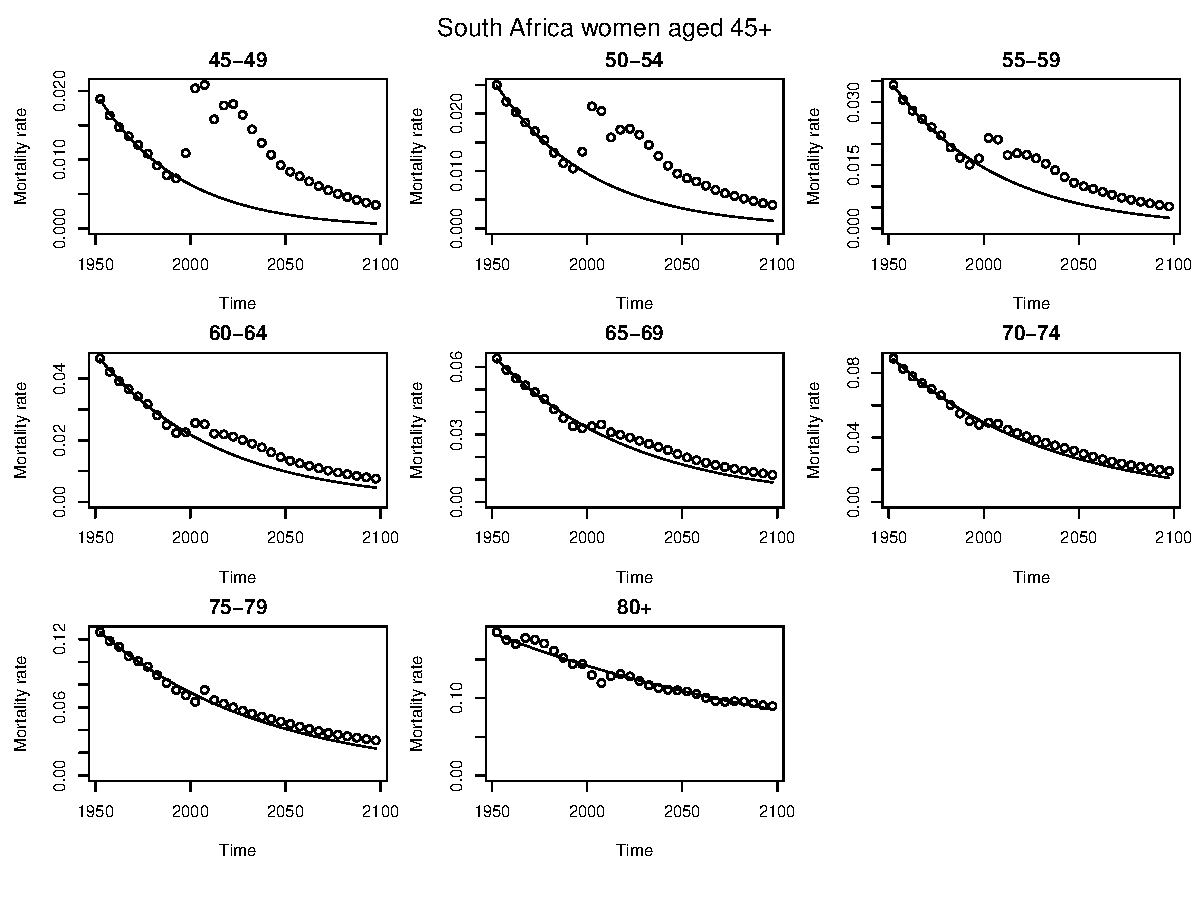
\includegraphics[width=16cm,height=16cm]{EstimatingRatesFromUNPD-MortalitySAWomen2} 

\caption{Mortality rates for women in South Africa over time by 5 year age groups (cont). Circles show UNPD estimates (including HIV mortality), lines show estimate based on a log-linear model for each age group.}
\label{MortalitySAmen1}
\end{figure}



\begin{figure}
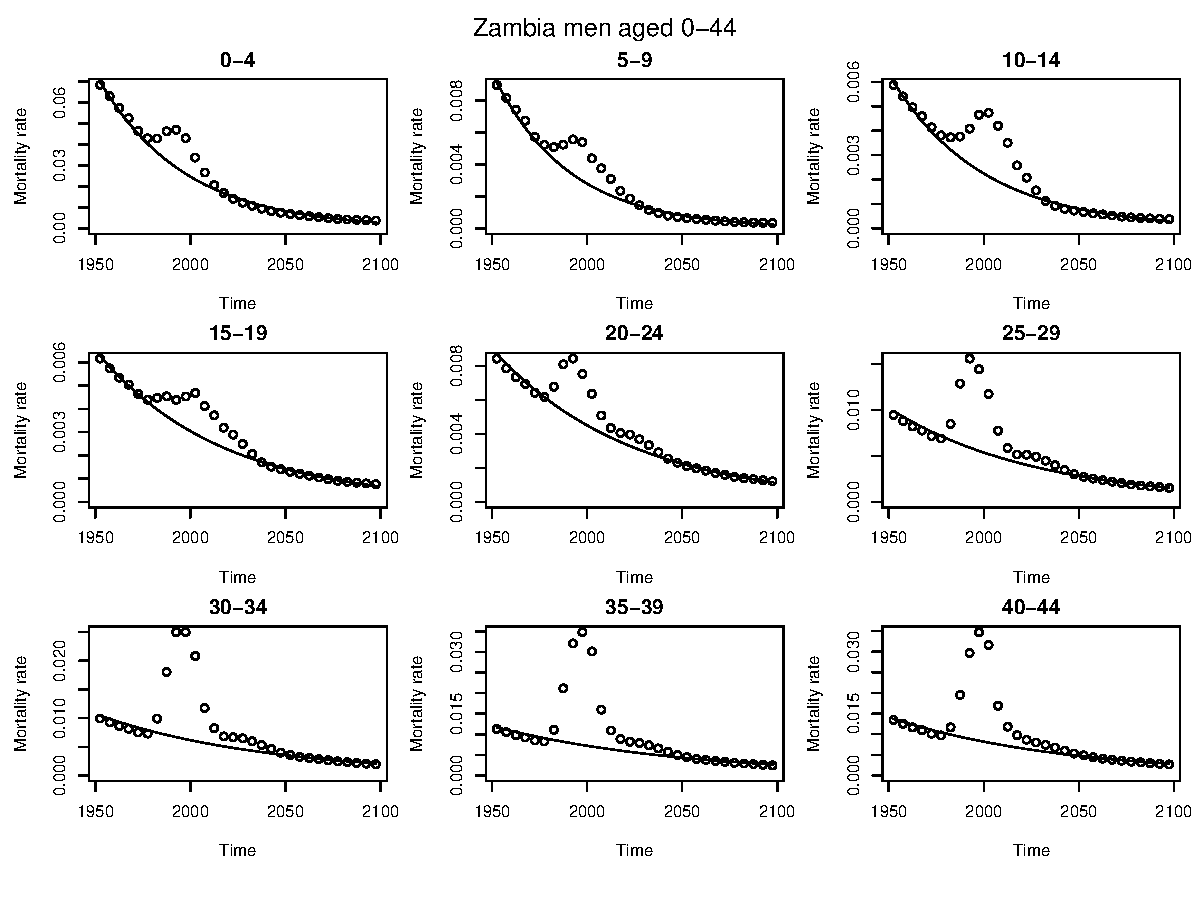
\includegraphics[width=16cm,height=16cm]{EstimatingRatesFromUNPD-MortalityZamMen1} 

\caption{Mortality rates for men in Zambia over time by 5 year age groups. Circles show UNPD estimates (including HIV mortality), lines show estimate based on a log-linear model for each age group.}
\label{MortalitySAmen1}
\end{figure}


\begin{figure}
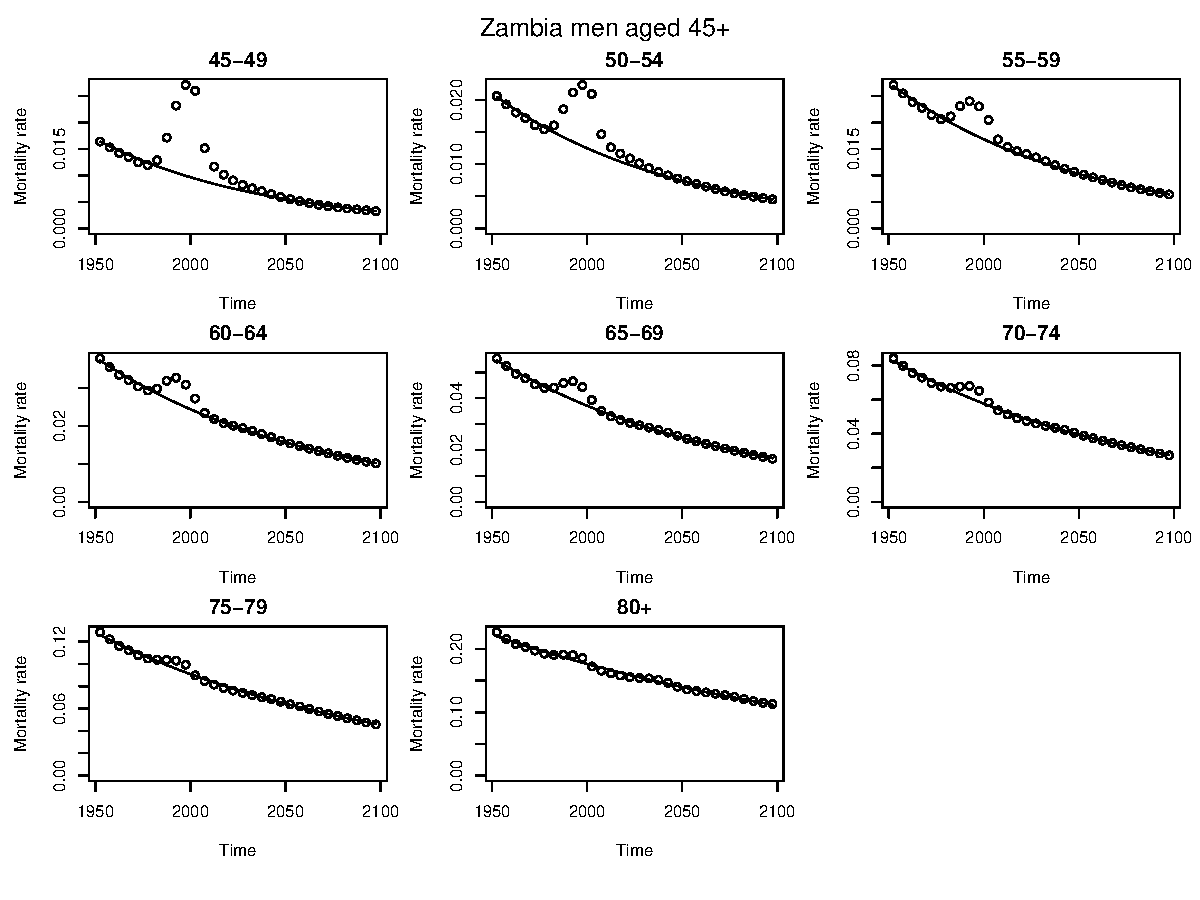
\includegraphics[width=16cm,height=16cm]{EstimatingRatesFromUNPD-MortalityZamMen2} 

\caption{Mortality rates for men in Zambia over time by 5 year age groups (cont). Circles show UNPD estimates (including HIV mortality), lines show estimate based on a log-linear model for each age group.}
\label{MortalitySAmen1}
\end{figure}


\begin{figure}
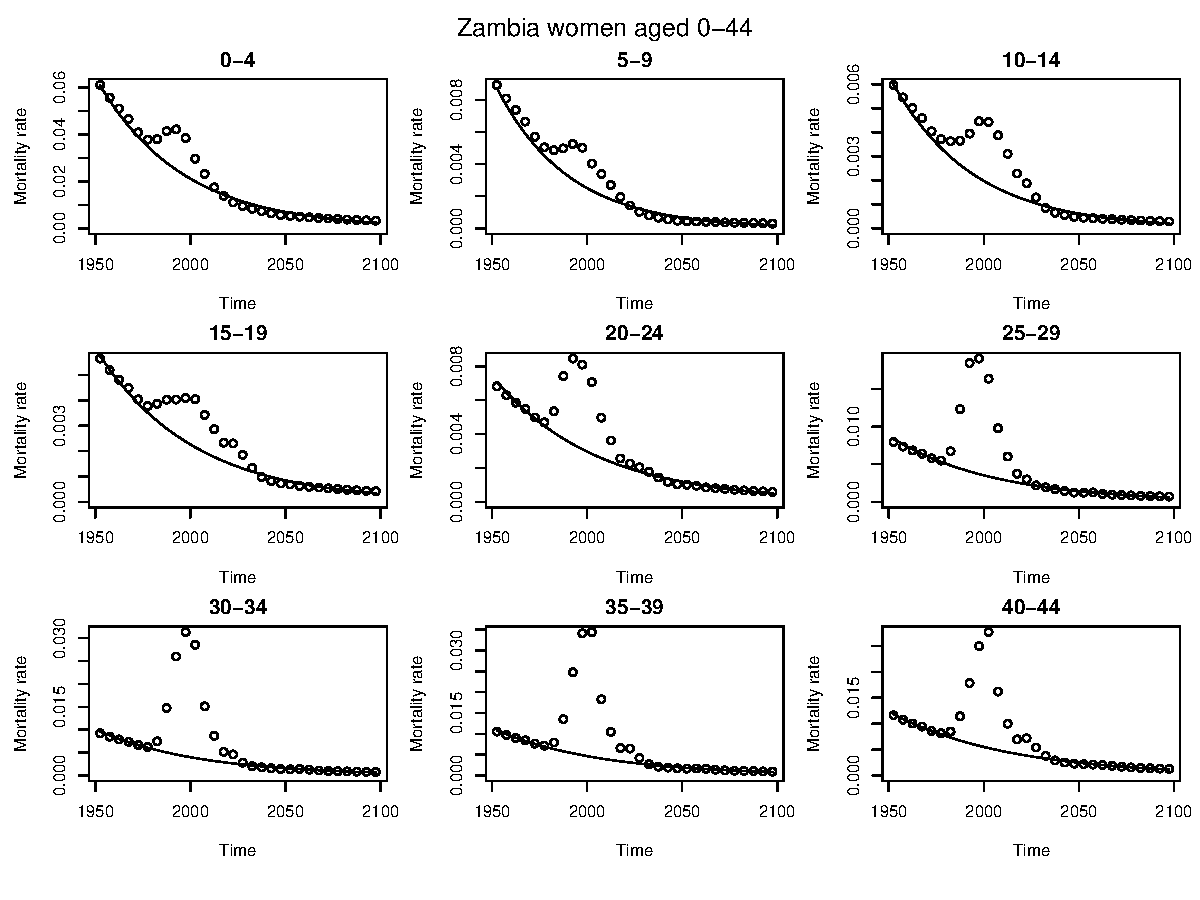
\includegraphics[width=16cm,height=16cm]{EstimatingRatesFromUNPD-MortalityZamWomen1} 

\caption{Mortality rates for women in Zambia over time by 5 year age groups. Circles show UNPD estimates (including HIV mortality), lines show estimate based on a log-linear model for each age group.}
\label{MortalitySAmen1}
\end{figure}


\begin{figure}
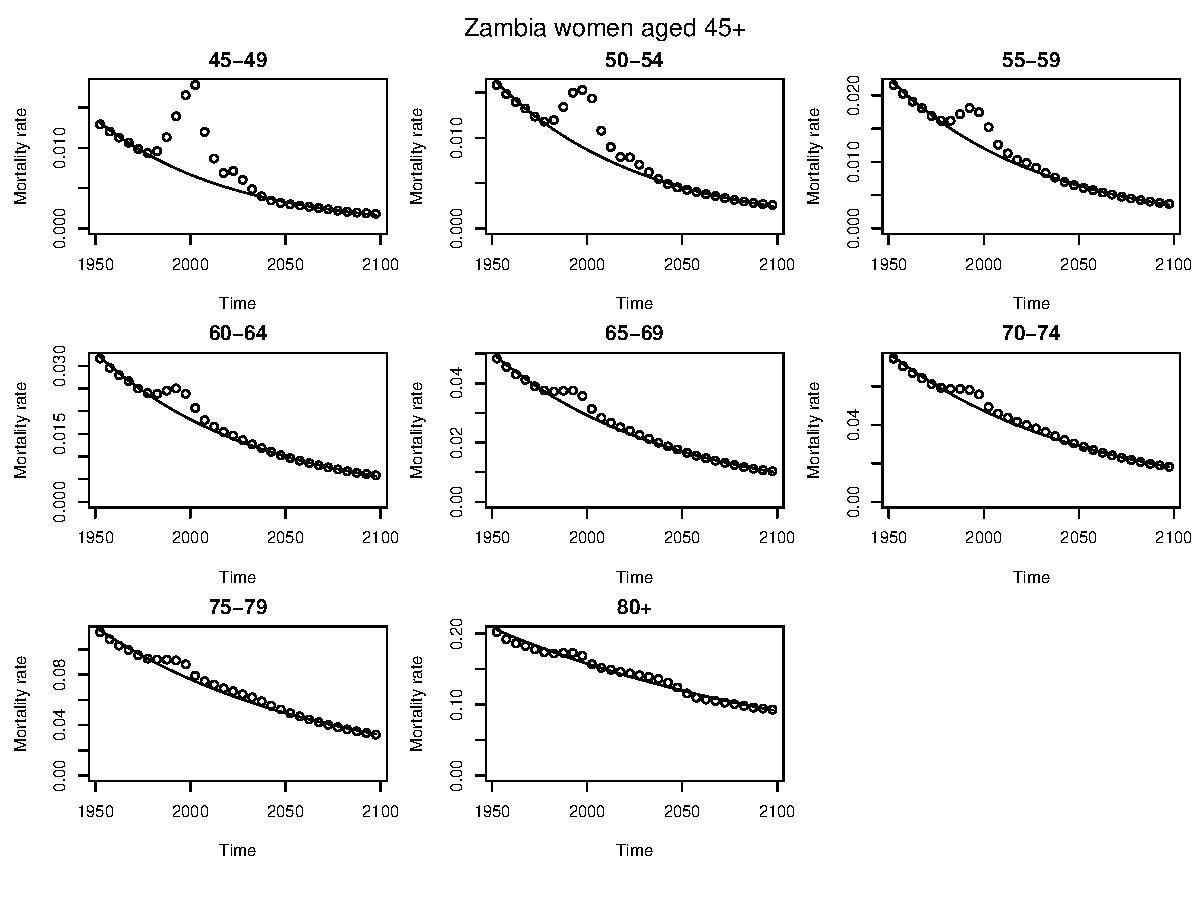
\includegraphics[width=16cm,height=16cm]{EstimatingRatesFromUNPD-MortalityZamWomen2} 

\caption{Mortality rates for women in Zambia over time by 5 year age groups (cont). Circles show UNPD estimates (including HIV mortality), lines show estimate based on a log-linear model for each age group.}
\label{MortalitySAmen1}
\end{figure}


\clearpage

\begin{landscape}
% latex table generated in R 3.6.0 by xtable 1.8-4 package
% Tue May 28 07:31:37 2019
\begin{table}[ht]
\centering
\begingroup\small
\begin{tabular}{rrrrrrrrrrrrrrrrrr}
  \hline
 & 0-4 & 5-9 & 10-14 & 15-19 & 20-24 & 25-29 & 30-34 & 35-39 & 40-44 & 45-49 & 50-54 & 55-59 & 60-64 & 65-69 & 70-74 & 75-79 & 80+ \\ 
  \hline
Intercept & 42.29 & 42.59 & 40.87 & 38.14 & 37.63 & 37.29 & 36.82 & 34.33 & 30.52 & 26.05 & 21.87 & 17.92 & 15.11 & 13.18 & 11.25 & 9.39 & 6.23 \\ 
  Coeff & -0.02 & -0.02 & -0.02 & -0.02 & -0.02 & -0.02 & -0.02 & -0.02 & -0.02 & -0.02 & -0.01 & -0.01 & -0.01 & -0.01 & -0.01 & -0.01 & -0.00 \\ 
   \hline
\end{tabular}
\endgroup
\caption{Parameters for South Africa men mortality} 
\end{table}% latex table generated in R 3.6.0 by xtable 1.8-4 package
% Tue May 28 07:31:37 2019
\begin{table}[ht]
\centering
\begingroup\small
\begin{tabular}{rrrrrrrrrrrrrrrrrr}
  \hline
 & 0-4 & 5-9 & 10-14 & 15-19 & 20-24 & 25-29 & 30-34 & 35-39 & 40-44 & 45-49 & 50-54 & 55-59 & 60-64 & 65-69 & 70-74 & 75-79 & 80+ \\ 
  \hline
Intercept & 54.69 & 68.21 & 69.07 & 71.72 & 71.85 & 68.58 & 63.58 & 56.24 & 47.61 & 40.42 & 35.67 & 31.79 & 27.90 & 24.09 & 21.63 & 20.42 & 8.48 \\ 
  Coeff & -0.03 & -0.04 & -0.04 & -0.04 & -0.04 & -0.04 & -0.03 & -0.03 & -0.03 & -0.02 & -0.02 & -0.02 & -0.02 & -0.01 & -0.01 & -0.01 & -0.01 \\ 
   \hline
\end{tabular}
\endgroup
\caption{Parameters for South Africa women mortality} 
\end{table}% latex table generated in R 3.6.0 by xtable 1.8-4 package
% Tue May 28 07:31:37 2019
\begin{table}[ht]
\centering
\begingroup\small
\begin{tabular}{rrrrrrrrrrrrrrrrrr}
  \hline
 & 0-4 & 5-9 & 10-14 & 15-19 & 20-24 & 25-29 & 30-34 & 35-39 & 40-44 & 45-49 & 50-54 & 55-59 & 60-64 & 65-69 & 70-74 & 75-79 & 80+ \\ 
  \hline
Intercept & 40.21 & 44.03 & 35.33 & 24.76 & 22.43 & 20.43 & 17.02 & 15.47 & 16.94 & 17.65 & 16.50 & 15.64 & 14.10 & 12.92 & 12.31 & 11.38 & 7.56 \\ 
  Coeff & -0.02 & -0.02 & -0.02 & -0.02 & -0.01 & -0.01 & -0.01 & -0.01 & -0.01 & -0.01 & -0.01 & -0.01 & -0.01 & -0.01 & -0.01 & -0.01 & -0.00 \\ 
   \hline
\end{tabular}
\endgroup
\caption{Parameters for Zambia men mortality} 
\end{table}% latex table generated in R 3.6.0 by xtable 1.8-4 package
% Tue May 28 07:31:37 2019
\begin{table}[ht]
\centering
\begingroup\small
\begin{tabular}{rrrrrrrrrrrrrrrrrr}
  \hline
 & 0-4 & 5-9 & 10-14 & 15-19 & 20-24 & 25-29 & 30-34 & 35-39 & 40-44 & 45-49 & 50-54 & 55-59 & 60-64 & 65-69 & 70-74 & 75-79 & 80+ \\ 
  \hline
Intercept & 40.71 & 46.71 & 40.58 & 33.24 & 30.93 & 30.74 & 31.50 & 30.23 & 27.04 & 23.51 & 21.27 & 20.79 & 19.76 & 18.14 & 16.55 & 14.73 & 9.20 \\ 
  Coeff & -0.02 & -0.03 & -0.02 & -0.02 & -0.02 & -0.02 & -0.02 & -0.02 & -0.02 & -0.01 & -0.01 & -0.01 & -0.01 & -0.01 & -0.01 & -0.01 & -0.01 \\ 
   \hline
\end{tabular}
\endgroup
\caption{Parameters for Zambia women mortality} 
\end{table}

\end{landscape}


%%%%%%%%%%%%%%%%%%%%%%%%%%%%%%%%%%%%%%%%%%%%%%%%
%
%%%%%%%%%%%%%%%%%%%%%%%%%%%%%%%%%%%%%%%%%%%%%%%%
\begin{Schunk}
\begin{Sinput}
> # Writing out mortality rates:
> write.table(rbind(mortality.coeffs.sa.men,mortality.coeffs.sa.women),file="SouthAfrica_mortalityByAgeCoefficients.txt",row.names=FALSE,col.names=FALSE)
> write.table(rbind(mortality.coeffs.zam.men,mortality.coeffs.zam.women),file="Zambia_mortalityByAgeCoefficients.txt",row.names=FALSE,col.names=FALSE)
> 
\end{Sinput}
\end{Schunk}

\clearpage

\section*{Fertility rates}





\begin{figure}
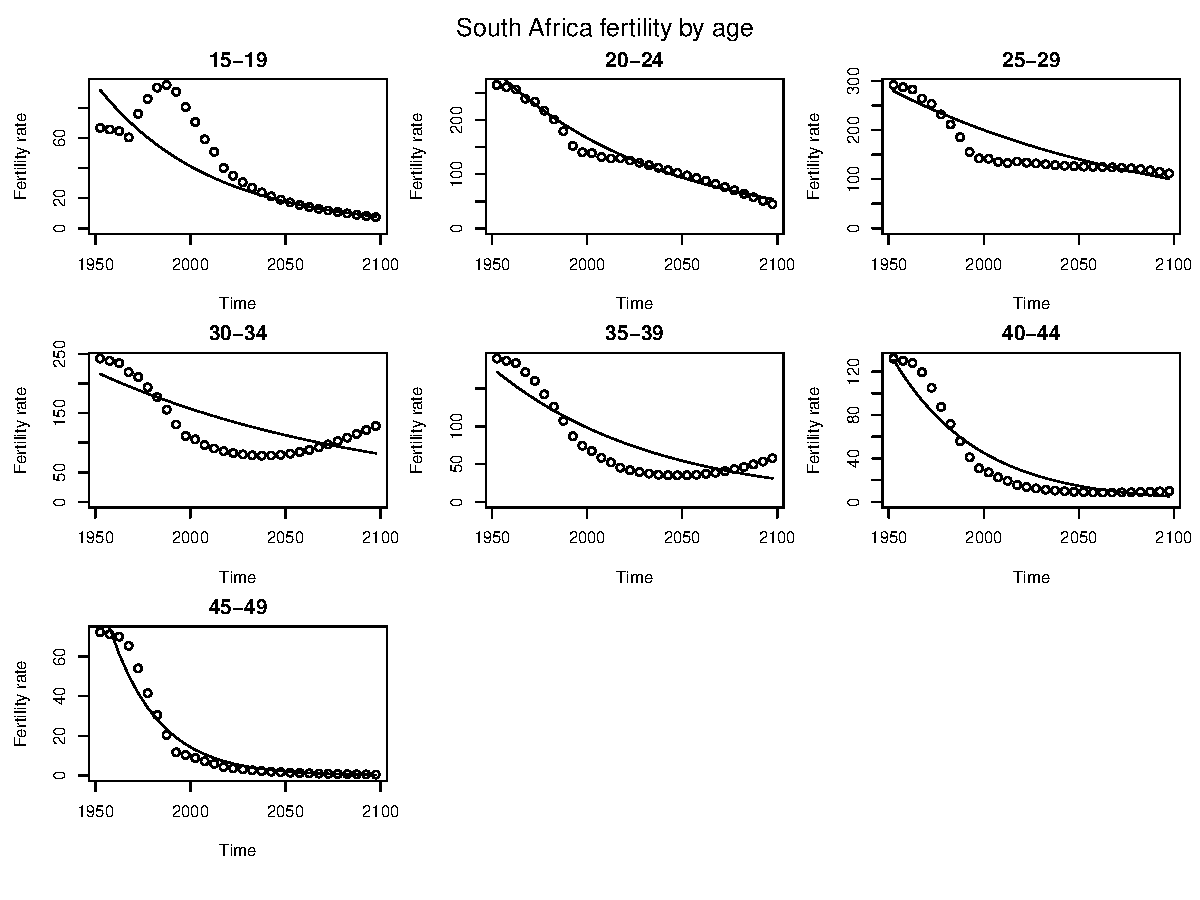
\includegraphics[width=16cm,height=16cm]{EstimatingRatesFromUNPD-FertilitySA} 

\caption{Fertility rates for women in South Africa over time by 5 year age groups. Circles show UNPD estimates (which are adjusted for the effects of HIV), lines show estimate based on a log-linear model for each age group.}
\label{FertilitySA}
\end{figure}

\begin{figure}
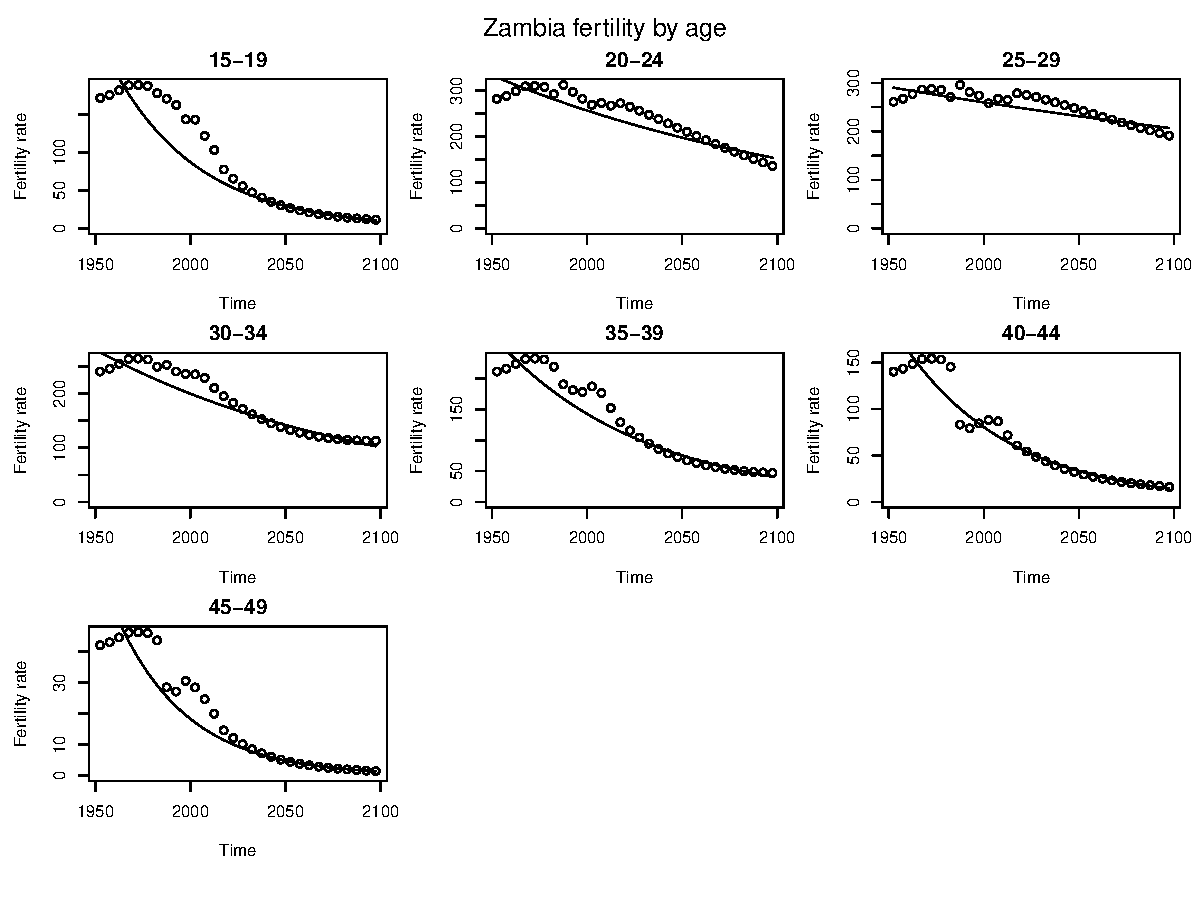
\includegraphics[width=16cm,height=16cm]{EstimatingRatesFromUNPD-FertilityZam} 

\caption{Fertility rates for women in Zambia over time by 5 year age groups. Circles show UNPD estimates (which are adjusted for the effects of HIV), lines show estimate based on a log-linear model for each age group.}
\label{FertilityZam}
\end{figure}



\clearpage
\section*{Experiments}
%%%%%%%%%%%%%%%%%%%%%%%%%%%%%%%%%%%%%%%%%%%%%%%%
% EXPERIMENT: Trying to see if a 2d function fits OK: 
%%%%%%%%%%%%%%%%%%%%%%%%%%%%%%%%%%%%%%%%%%%%%%%%

\begin{figure}
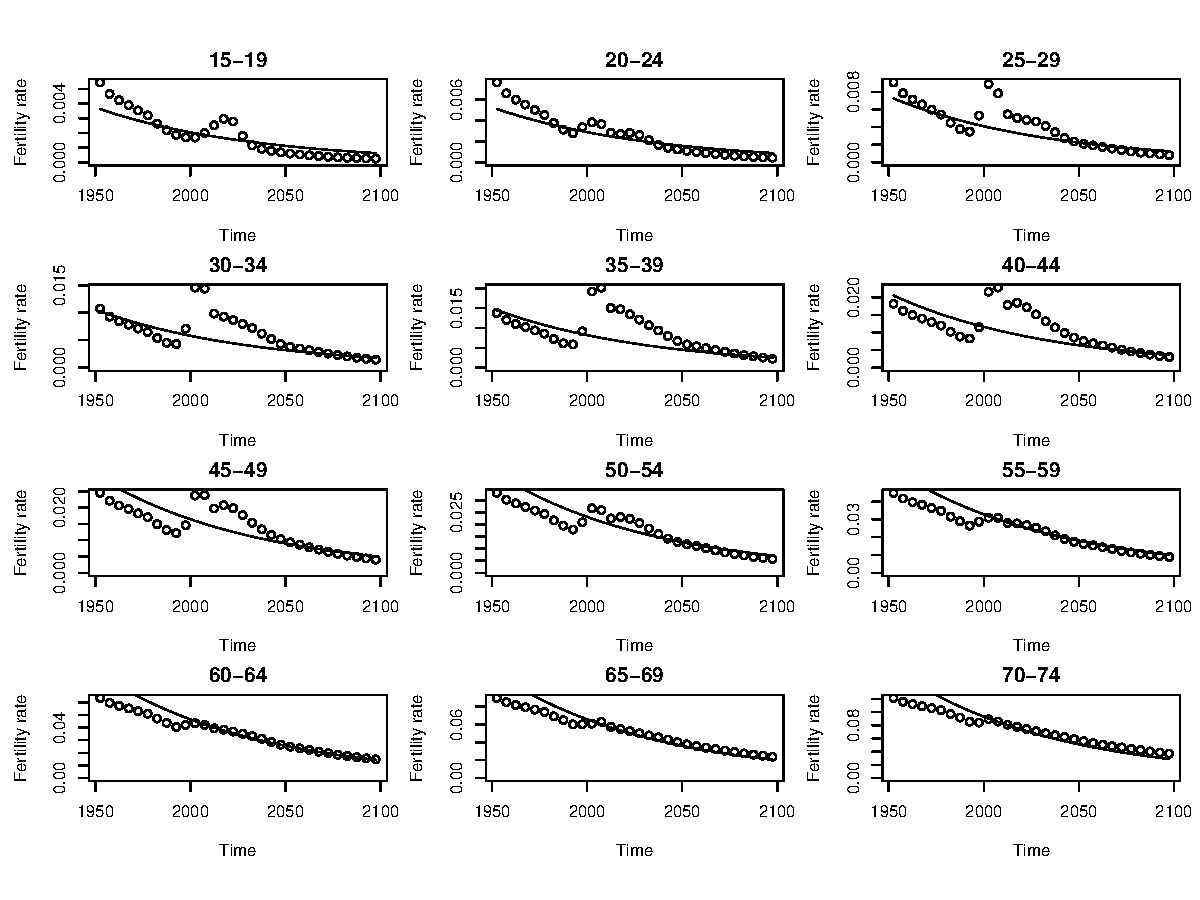
\includegraphics[width=16cm,height=16cm]{EstimatingRatesFromUNPD-TestSAmortality2d} 

\caption{Experiment for SA men to see if we can fit a 2d function - ie a single regression by age group and time for each gender and country -  well for mortality. For now I think we should stick with the different regressions for each age group.}
\label{FertilityZam}
\end{figure}

\section*{Discussion}

For mortality rates we need to have some way of discounting HIV mortality. I think that fitting a function separately to each age group  - and ignoring the periods when HIV mortality is high - gives an OK fit. It seems to me that we can't fit a 2d model by age and time (assuming independence between the 2) as well. As mortality is something in the background, validated against age distribution at different time points, I think we can ignore the parametric complexity and just input them as fixed quantities.

For fertility it is not clear that any function will fit this well. For now we can use the UNPD numbers directly.

\end{document}
